\documentclass{beamer}

\usetheme{Boadilla}

\usepackage[utf8]{inputenc}
\usepackage{listings}

\title{Installieren von Python}
\subtitle{in verschiedenen Operating Systems}
\author{Felix V.}
\date{\today}

\lstset{
  backgroundcolor=\color{black},
  basicstyle=\color{green}
}   

\begin{document}
\begin{frame}
\titlepage
\end{frame}

\begin{frame}
  \frametitle{Was wir heute noch machen}
  \tableofcontents  
\end{frame}
\section{Installation unter Windows}
\subsection{Download für Windows}
\begin{frame}
  \frametitle{Installation unter Windows}
  \framesubtitle{Download für Windows}
  \url{https://www.python.org}
\end{frame}
\begin{frame}
  \frametitle{Download für Windows}
  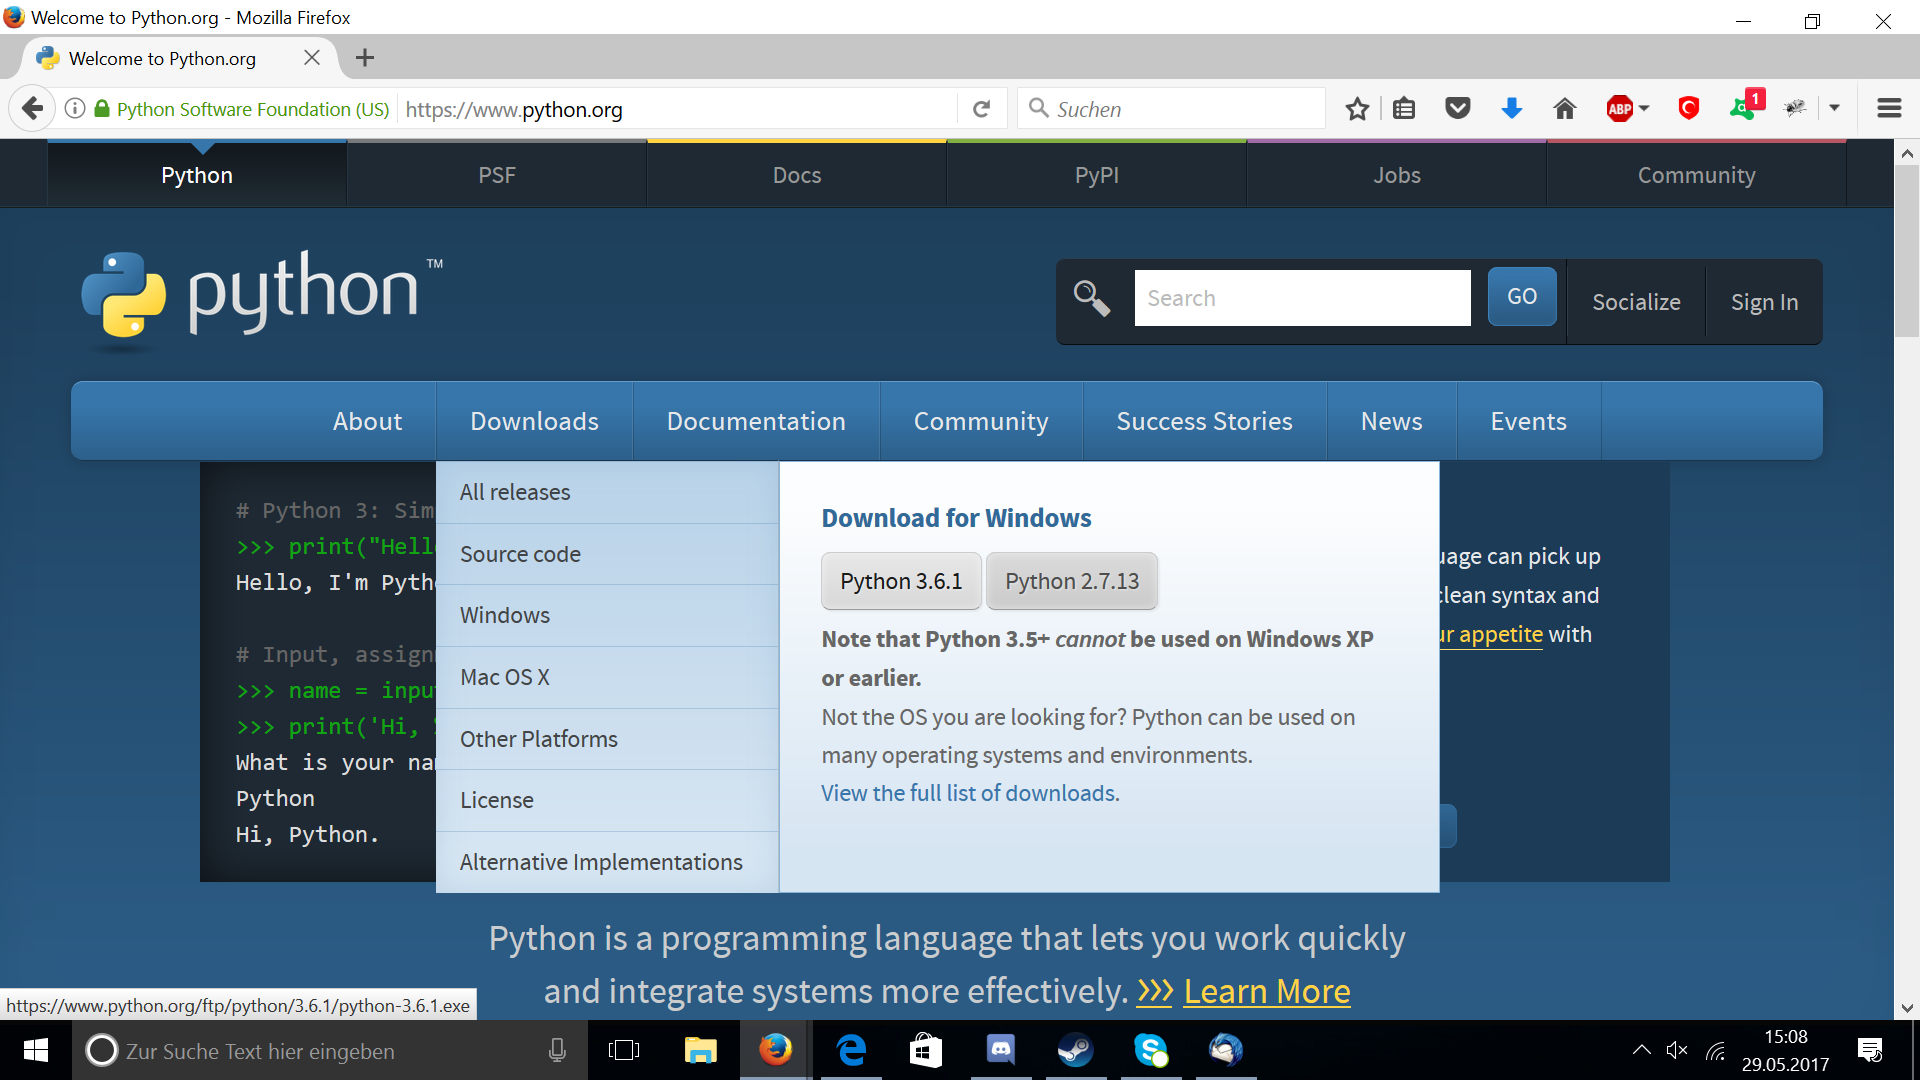
\includegraphics[width=\textwidth]{./screenshotWin0.png}
\end{frame}
\begin{frame}
  \frametitle{Installation für Windows}
  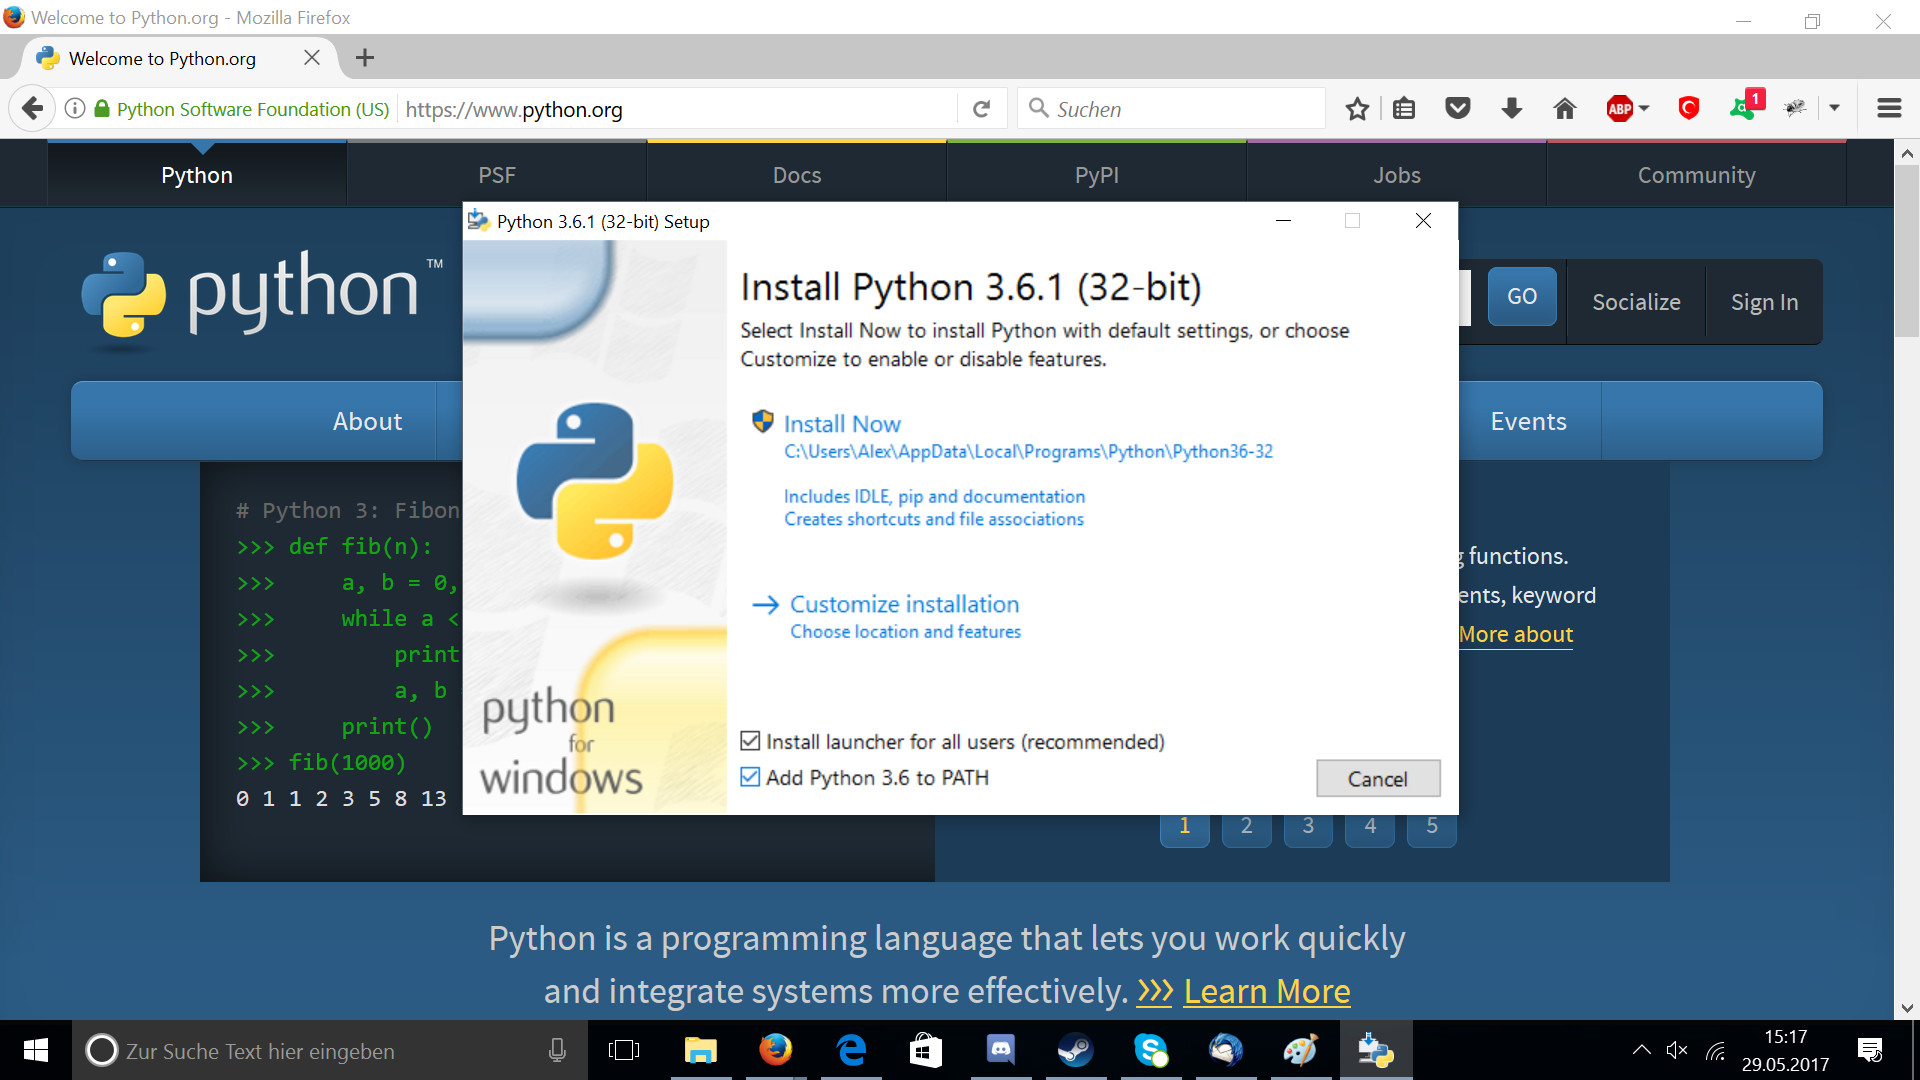
\includegraphics[width=\textwidth]{./screenshotWin1.png}
\end{frame}
\section{Installation unter Linux Debian/Ubuntu/Linux Mint}
\begin{frame}[fragile]
  \frametitle{Installation unter Linux Debian/Ubuntu/Linux Mint}
  \begin{lstlisting}[numbers=none]
    $ sudo apt-get install python3 python3-pip
  \end{lstlisting}
\end{frame}
\section{Installation unter Arch Linux/Manjaro}
\begin{frame}[fragile]
  \frametitle{Installation unter Arch Linux/Manjaro}
  \begin{lstlisting}[numbers=none]
    $ sudo pacman -S install python3 python3-pip
  \end{lstlisting}
\end{frame}
\section{Installation unter OSX}
\begin{frame}
  \frametitle{Installation unter OSX}
  \begin{itemize}
    \item homebrew
    \item Mac OS X 64-bit/32-bit installer auf python.org $->$ Downloads $->$ OSX
  \end{itemize}
\end{frame}
\section{Sonstige interessante Software}
\begin{frame}
  \frametitle{Sonstige software}
  \begin{itemize}
  \item numpy, scipy, matplotlib
  \item IDLE
  \item editor (Atom, Emacs und Vim habe gute Erweiterungen)
  \item IPython
  \item spider2,spider3,eric
  \item nicht freie Software
    \begin{itemize}
    \item sublimeText3 (und auch 2)
    \item pycharm von JetBrains
    \end{itemize}
  \item flask, django, pandas
  \end{itemize}
\end{frame}


\end{document}

%%% Local Variables:
%%% mode: latex
%%% coding: utf-8
%%% TeX-master: t
%%% End:
%vim:fdm=marker set ft=tex: